\chapter{Computer-Aided Drug Discovery}

In the modern drug discovery pipeline, two early stages are lead identification and lead optimization. From the computational perspective, lead identification can be addressed by virtual screening, while lead optimization can be addressed by computational ligand synthesis.

\section{Protein-Ligand Docking}

As the X-ray crystallography and Nuclear Magnetic Resonance (NMR) technologies evolve, more and more 3D structures of biological macromolecules at atomic level have been revealed and deposited into the world's largest repository PDB (Protein Data Bank) \citep{540,537}. This rapid evolution catalyzes the development of various algorithms and tools for structure-based drug discovery via protein-ligand docking.

Protein-ligand docking is a method which predicts the preferred conformation (i.e. position and orientation) of a small ligand when bound to a macro protein to form a stable complex (Figure \ref{Background:Docking}, reprinted from Wikipedia). It also predicts the binding affinity in terms of free energy, which is basically the overall effect of various chemical forces involved, such as van der Waals force, electrostatic force, hydrogen bonding, hydrophobic interactions, Pi-Pi interactions, and the like. Free energy measures the degree of freedom of the ligand to ``escape'' from the protein, so the lower the free energy, the higher the binding affinity. Very often, the target protein is a viral enzyme of interest, and the small organic ligands that are predicted to inhibit the viral enzyme are what we want to discover.

\begin{figure}
\centering
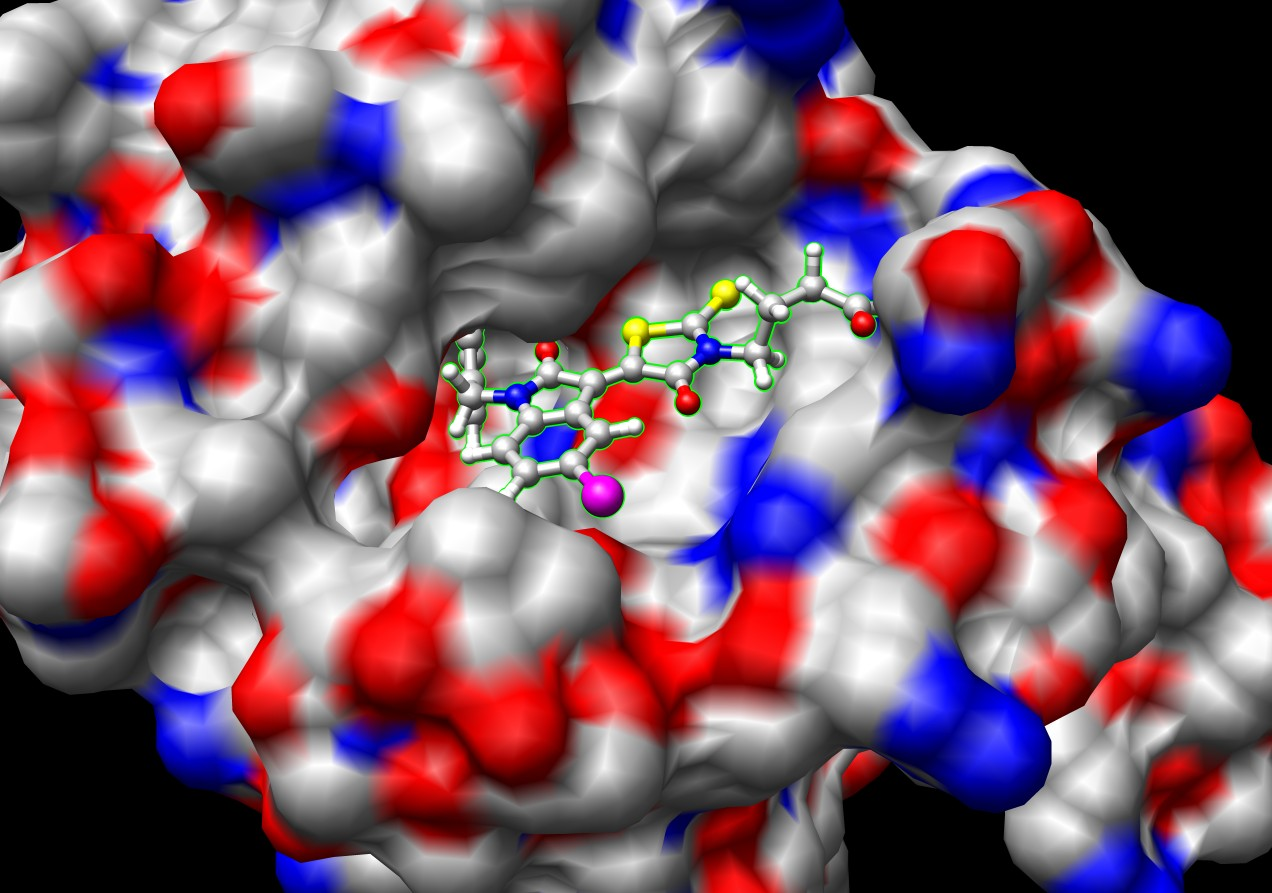
\includegraphics[width=\textwidth]{Background/Docking.jpg}
\caption{A ligand docked against a protein. Source: Wikipedia.}
\label{Background:Docking}
\end{figure}

Docking programs typically consist of two basic components, a scoring function to predict the binding affinity, and an algorithm to explore the conformational space of the ligand and the protein \citep{493}. So far, dozens of scoring functions \citep{579,566,570,775,575,576,578,580,581,774} and dozens of algorithms \citep{595,564,594,602,603,604,605,606,607,781,614,615,617} have been developed. Some methods have been comprehensively evaluated and compared \citep{637,771,556}.

Among the many docking programs, AutoDock Vina \citep{595} (hereafter Vina for short) is a competitive one. It's free and open source. It runs faster than its predecessor AutoDock 4 \citep{596} by an order of magnitude \citep{556}. Released in 2010, Vina has been cited by 117 other publications and adopted by many researchers \citep{609}. Indeed, it is intensively used in our research projects too.

Virtual screening is simply a massive version of docking (Figure \ref{Background:VirtualScreening} \citep{470}). It docks a database of drug-like ligands to a viral protein of interest, ranks them according to their predicted binding affinity, and shortlists the best ones for further investigation. Statistical frameworks and assessments have been established for evaluation and result selection \citep{489,491,769,583,582}. In reality, docking and virtual screening have successful applications for drug discovery \citep{495,498,751,503,752,757,506,738,761,763,766,736}.

\begin{figure}
\centering
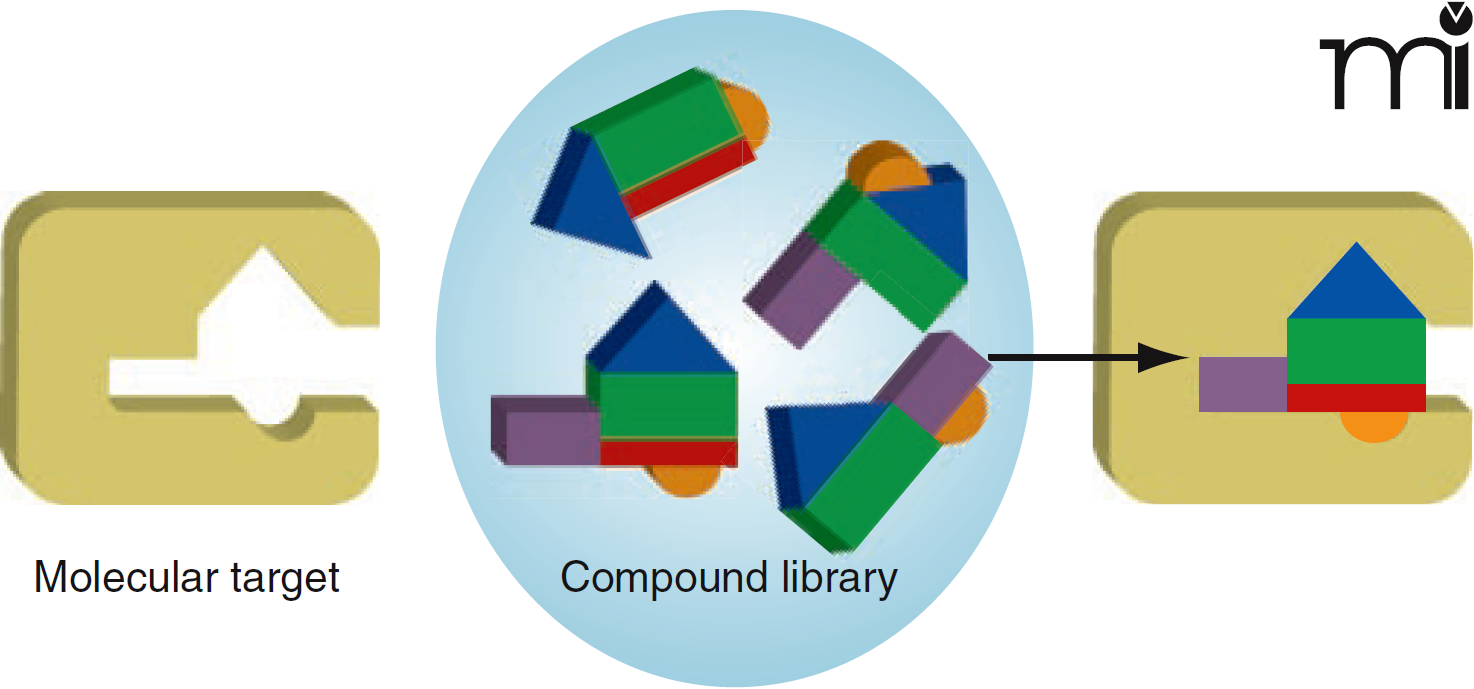
\includegraphics[width=\textwidth]{Background/VirtualScreening.png}
\caption{Virtual screening to identify compounds that bind to the target. Figure reprinted from \citep{470}.}
\label{Background:VirtualScreening}
\end{figure}

There are quite a lot data sources and databases for virtual screening, such as PDB \citep{540,537}, ZINC \citep{532}, PDBbind \citep{529,530}, and PubChem \citep{526}. In addition to raw data, there are library analysis \citep{521}, benchmark datasets \citep{534,533,535,536}, and data manipulation tools \citep{542}. Some tools exploit massive parallelism in the form of either cluster computing or cloud computing \citep{557,773,560,782}.

%Scoring function
%Efficiency index \citep{335,336,337}

%Drug properties
%ADMET \citep{325,326,327,328,329,330,331,332}
%Others \citep{333,334}
%Drug-Drug Interactions \citep{338}
%LogP \citep{341,342,343,344,345,346}
%pKa \citep{347,348}

\section{Ligand Synthesis}

Virtual screening tries to discover promising ligands out of existing databases. Apparently the diversity of its outcome is limited to the diversity of the database. In other words, virtual screening will fail if the database contains no promising ligands at all.

In contrast, computational synthesis produces novel molecular structures with desired pharmacological properties. It helps to explore a much larger chemical space for novel drugs. Figure \ref{igrow:LigandDesign} \citep{363} illustrates three kinds of strategies for ligand design. A number of compounds that evolved from fragments have entered the clinic, and the approach is increasingly accepted as an additional route to identifying new hits in inhibitor design \citep{363,470}.

\begin{figure}[t]
\centering
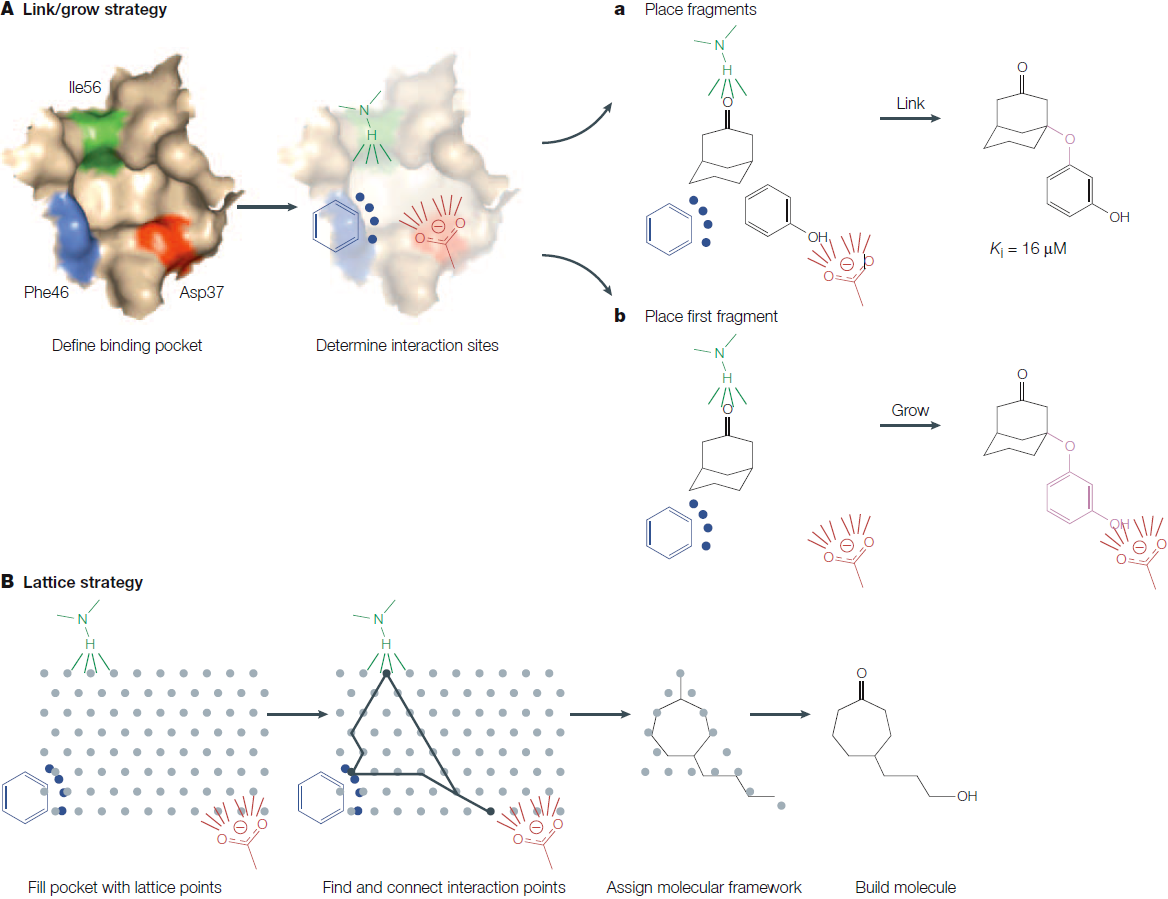
\includegraphics[width=\textwidth]{igrow/LigandDesign.png}
\caption{Ligand design strategies. Figure reprinted from \citep{363}.}
\label{igrow:LigandDesign}
\end{figure}

A computational synthesis program is confronted with a virtually infinite search space. The number of chemically feasible, drug-like molecules has been estimated to be in the order of 10\textsuperscript{60} to 10\textsuperscript{100} \citep{363}, from which the most promising candidates have to be selected and synthesized. Rather than the systematic construction and evaluation of each individual compound, computational synthesis programs rely on the principle of local optimization, which does not necessarily lead to the globally optimal solution. In fact, most software implementations \citep{466,749} are non-deterministic, and rely on some kind of stochastic structure optimization.

Among the many ligand synthesis programs, AutoGrow \citep{466} is a representative one which implements genetic algorithm to create a population of ligands. It is the only ligand synthesis program that uses Vina \citep{595} as external docking engine for the selection operator. It is free and open source. However, it requires messy configurations and its performance is hardly considered to be amazing. Hence its user base is rather limited and has been cited by merely 8 other publications since it was born in 2009. It is used as a baseline tool in our research projects.

\section{General-Purpose Computing on GPU}

The modern GPU has evolved from a fixed-function graphics pipeline to a programmable parallel processor with extremely high computational throughput and tremendous memory bandwidth at an affordable price. The past 5 years have seen a fruitful of algorithms for computer-aided drug discovery being ported to the GPU and gaining orders of magnitude of speedup over single threaded CPU counterparts. To name a few, such GPU-accelerated applications include binding site mapping \citep{722}, protein database search \citep{189}, compound selection \citep{750}, molecular docking \citep{723,652,779}, chemical similarity calculation \citep{726}.

As of June 2012, NVIDIA’s latest GPU architecture is codenamed ``Kepler" with its full implementation codenamed ``GK104", while AMD's latest GPU architecture is codenamed ``Southern Islands" with its full implementation codenamed ``Tahiti".

\subsection{NVIDIA GK104 and CUDA}

From the hardware perspective, the GK104-based GeForce GTX 680 GPU features 3.09 TFLOPS single-precision computing power and 128 GFLOPS double-precision computing power, 2GB GDDR5 memory with a bandwidth of 192GB/s, and a TDP (Thermal Design Power) of 195W.

Figure \ref{GPU:GeForceGTX680BlockDiagram} shows the block diagram of GeForce GTX 680, which consists of 4 GPCs (Graphics Processing Clusters), each having a dedicated raster engine and 2 SMX (next-generation Streaming Multiprocessors) units. With a total of 8 SMX units, the GeForce GTX 680 has 1536 CUDA Cores.

\begin{figure}
\centering
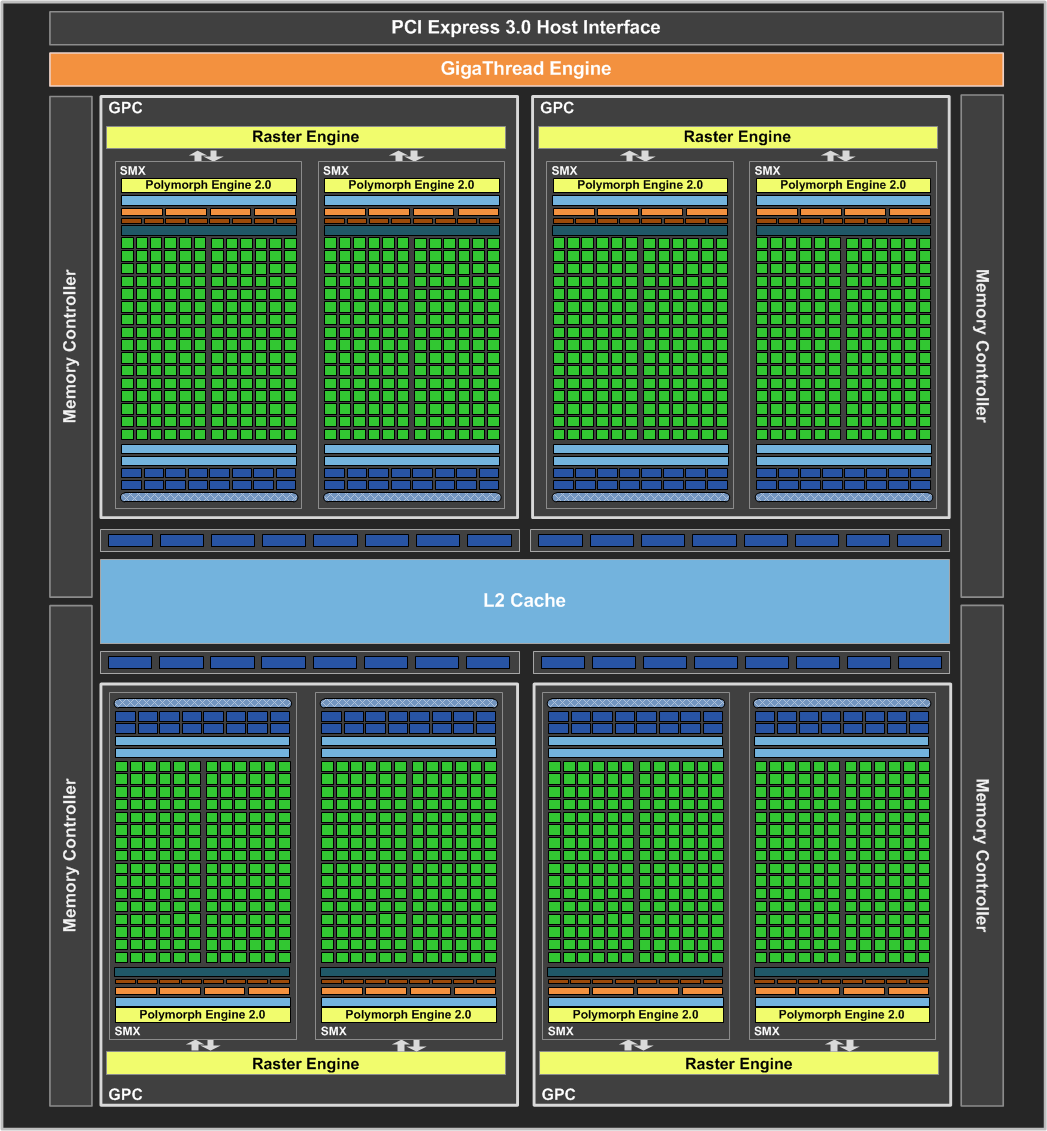
\includegraphics[width=\textwidth]{GPU/GeForceGTX680BlockDiagram.png}
\caption{NVIDIA GeForce GTX680 block diagram. Source: NVIDIA.}
\label{GPU:GeForceGTX680BlockDiagram}
\end{figure}

Figure \ref{GPU:GeForceGTX680SMX} shows the block diagram of GK104 SMX unit, which features 192 IEEE 754-2008 compliant single-precision CUDA cores, 32 SFUs (Special Function Units), 4 warp schedulers, 8 instruction dispatch units, and 64KB of configurable shared memory / L1 cache. Each CUDA core has fully pipelined floating-point and integer arithmetic logic units, while the SFUs handle fast approximate transcendental and graphics interpolation instructions.

The SMX schedules threads in groups of 32 parallel threads called warps. The 4 warp schedulers allow 4 warps to be issued and executed concurrently. Each warp scheduler is capable of dispatching 2 instructions per warp every clock in order to feed the execution resources of SMX.

\begin{figure}
\centering
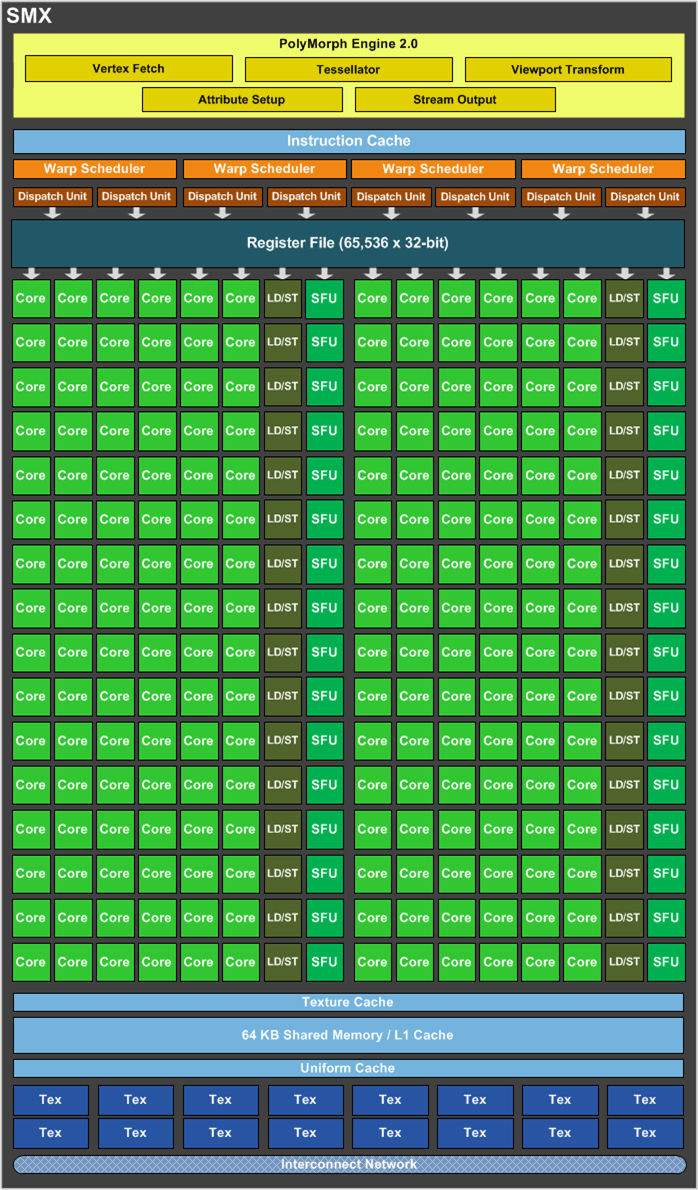
\includegraphics[width=\textwidth]{GPU/GeForceGTX680SMX.png}
\caption{NVIDIA GeForce GTX680 SMX. Source: NVIDIA.}
\label{GPU:GeForceGTX680SMX}
\end{figure}

From the software perspective, the GeForce GTX 680 supports CUDA (Compute United Device Architecture) 4.2, and thus can execute programs written in C, C++, Fortran, and other languages. A CUDA program invokes functions called kernels that execute across parallel CUDA threads, which are organized into thread blocks and grids of thread blocks. The hierarchy of CUDA threads maps to the hierarchy of CUDA cores on the GPU; a GPU executes one or more grids; an SMX executes one or more thread blocks; and CUDA cores and other execution units in the SMX execute thread instructions from kernel compilation.

Figure \ref{GPU:CUDAMemoryHierarchy} shows the CUDA hierarchy of threads, blocks and grids, and their corresponding memory space. A CUDA thread within a thread block maintains a program counter and executes an instance of the kernel. It has a per-thread private memory space used for register spills, function calls, and C automatic array variables. A thread block is a set of concurrently executing threads that can cooperate among themselves through barrier synchronization and shared memory. It has a per-block shared memory space used for inter-thread communication, data sharing, and result sharing. A grid is an array of thread blocks that execute the same kernel, read inputs from global memory, write results to global memory, and synchronize between dependent kernel calls. Grids share results in global memory after kernel-wide synchronization.

\begin{figure}
\centering
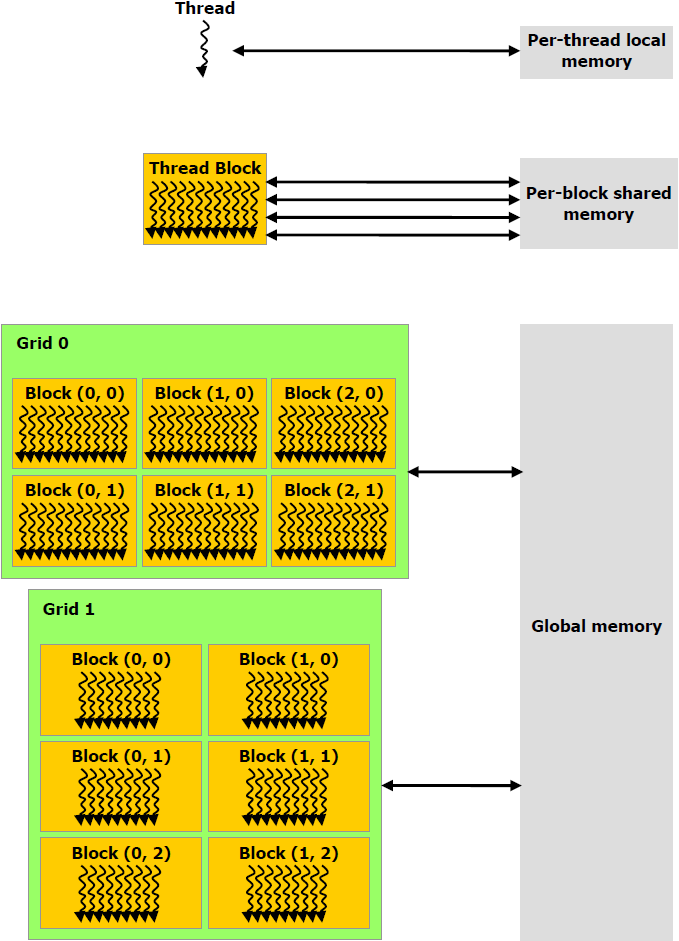
\includegraphics[width=\textwidth]{GPU/CUDAMemoryHierarchy.png}
\caption{CUDA hierarchy of threads, blocks, and grids, with corresponding per-thread private, per-block shared, and per-application global memory spaces. Source: NVIDIA.}
\label{GPU:CUDAMemoryHierarchy}
\end{figure}

\subsection{AMD Tahiti and OpenCL}

From the hardware perspective, the Tahiti-based Radeon HD 7970 GPU features 3.79 TFLOPS single-precision computing power and 947 GFLOPS double-precision computing power, 3GB GDDR5 memory with a bandwidth of 264GB/s, and a TDP of 250W.

Figure \ref{GPU:RadeonHD7970BlockDiagram} shows the block diagram of Radeon HD 7970, which consists of 32 GCN (Graphics Core Next) cores, each heaving 64 stream processors, translating to a total of 2048 stream processors.

\begin{figure}
\centering
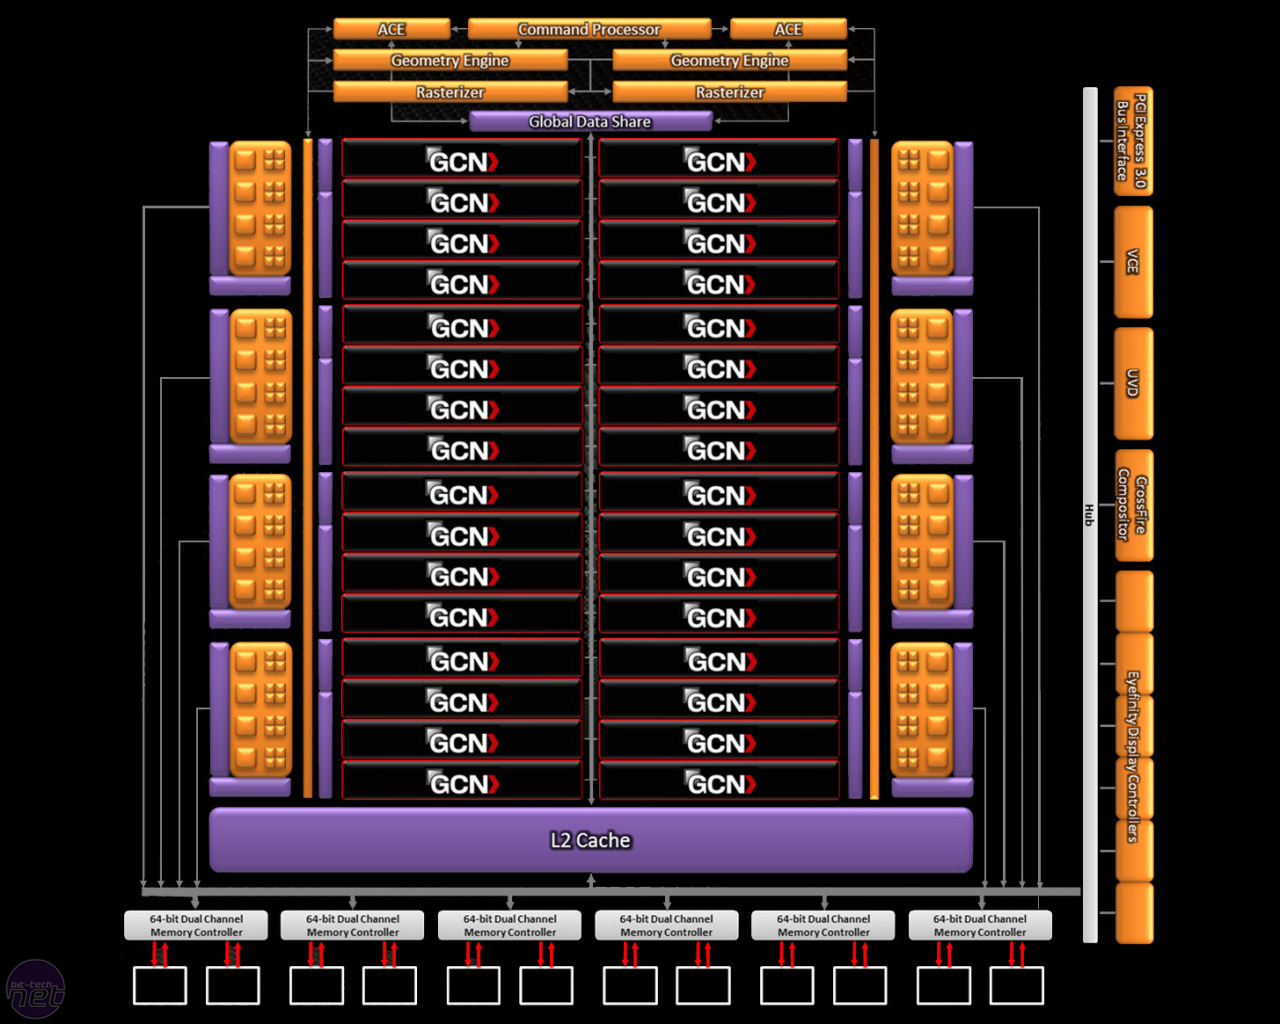
\includegraphics[width=\textwidth]{GPU/RadeonHD7970BlockDiagram.jpg}
\caption{AMD Radeon HD 7970 block diagram. Source: AMD.}
\label{GPU:RadeonHD7970BlockDiagram}
\end{figure}

Figure \ref{GPU:RadeonHD7970GCN} shows the block diagram of a GCN core, which features a scheduler, 4 SIMD-16 vector units, 4 64KB vector registers, a single scalar unit, 64KB of LDS (Local Data Share), and 16KB of L1 cache. The GCN core schedules threads in groups of 16 parallel threads called wavefronts. The 4 SIMD-16 vector units are capable of not only processing 4 wavefronts in 4 clock cycles, equivalent to one wavefront per cycle, but also handling special functions like transcendentals at a rate of 4 operations per clock cycle. The scalar unit assists with flow control and handles address generation for pointers. The L1 cache has an aggregate bandwidth of about 2 TB/s.

\begin{figure}
\centering
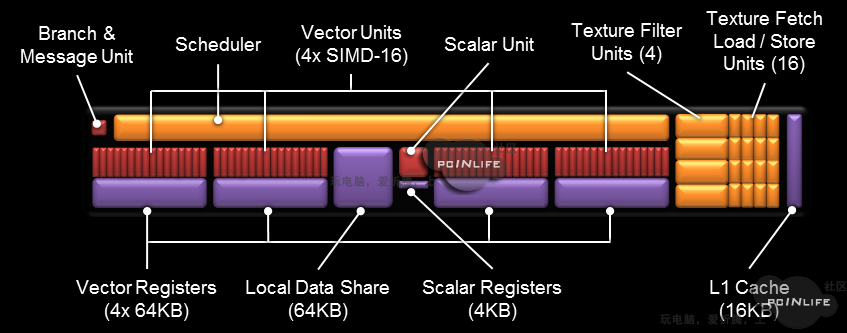
\includegraphics[width=\textwidth]{GPU/RadeonHD7970GCN.png}
\caption{AMD Radeon HD 7970 GCN. Source: AMD.}
\label{GPU:RadeonHD7970GCN}
\end{figure}

Figure \ref{GPU:RadeonHD7970CacheHierarchy} shows the cache hierarchy of Radeon HD 7970. A group of 4 GCN cores shares a 16KB instruction cache and a 32KB scalar data cache. The GDS (Global Data Share) enables L1 cache synchronization across all the GCN cores, which communicate over a shared bus to 6 128KB L2 cache partitions, each associated with a 64-bit dual-channel memory controllers, for a total of 768KB of L2 cache. The L2 cache can transfer nearly 710GB/s at 925MHz.

\begin{figure}
\centering
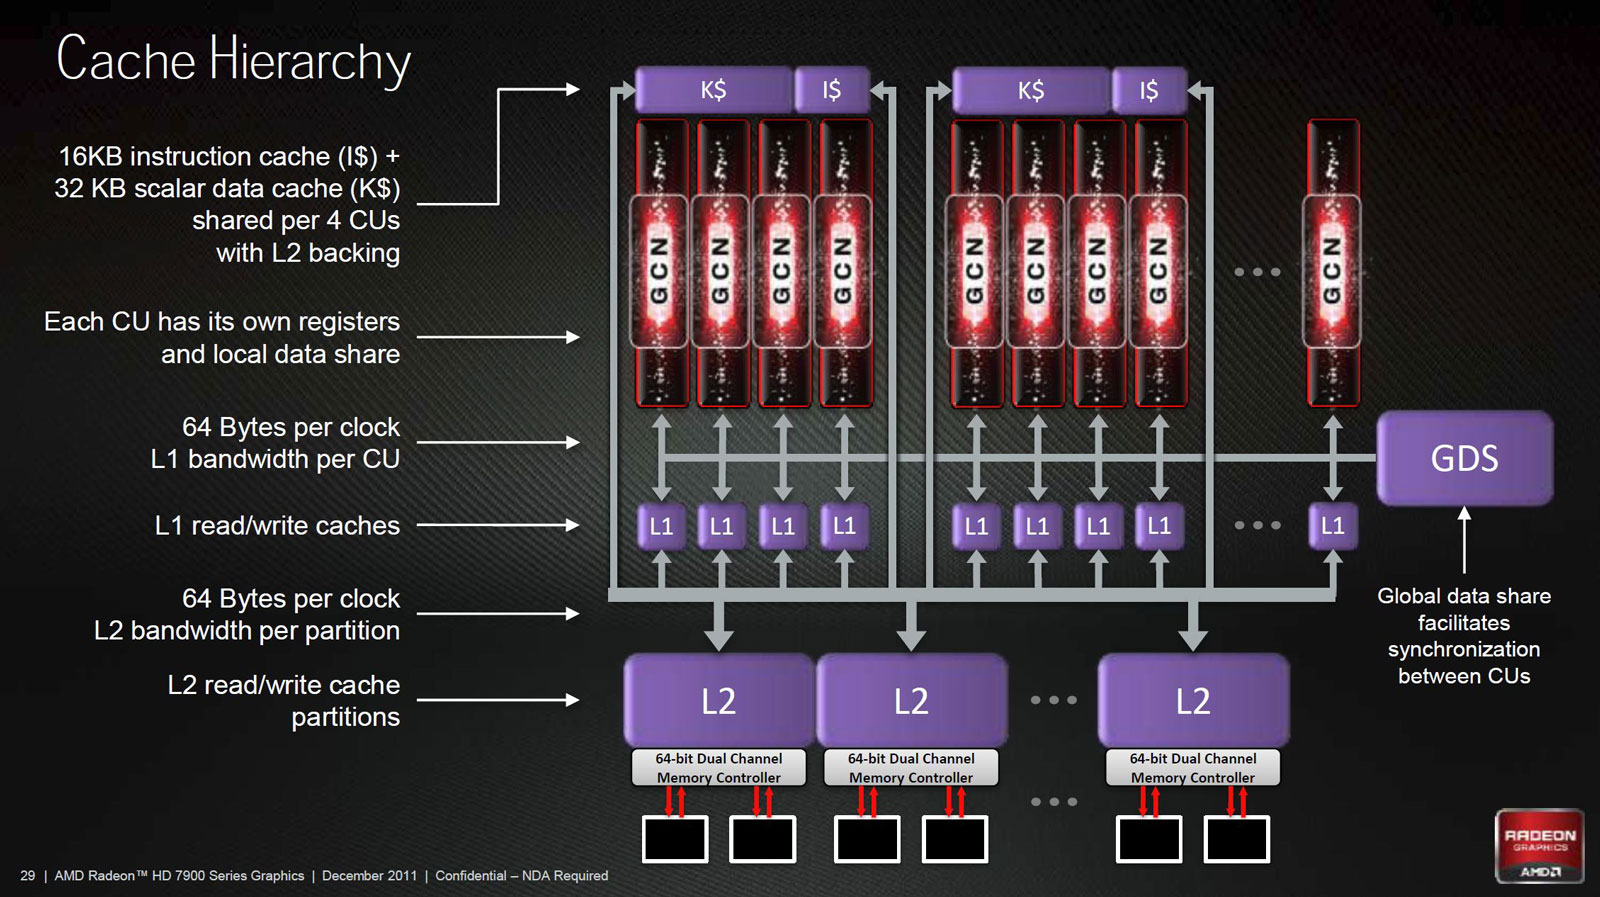
\includegraphics[width=\textwidth]{GPU/RadeonHD7970CacheHierarchy.jpg}
\caption{AMD Radeon HD 7970 cache hierarchy. Source: AMD.}
\label{GPU:RadeonHD7970CacheHierarchy}
\end{figure}

From the software perspective, the Radeon HD 7970 supports OpenCL (Open Computing Language) 1.2, and thus can execute programs written in C. There is a C++ wrapper for OpenCL 1.1. An OpenCL program invokes functions called kernels that execute across parallel work-items, which are organized into work-groups. The hierarchy of work-items maps to the hierarchy of stream processors on the GPU; a GPU executes one or more kernels; a GCN core executes one or more work-groups; and stream processors execute work-item instructions from kernel compilation.

Portability is the distinct feature that distinguishes OpenCL from CUDA. Multiple conformant implementations from AMD, NVIDIA, Intel, IBM, and embedded device vendors are shipping, fulfilling the philosophy of ``write once, execute everywhere".

\section{Software as a Service}

Ten Simple Rules for Getting Ahead as a Computational Biologist. Make software and website count \citep{260}
Ten Simple Rules for Providing a Scientific Web Resource \citep{677}
DOCK BLASTER
wwLigCSRre
ZINCPharmer

\chapterend
